\documentclass{scrreprt}
% Language
\usepackage[utf8]{inputenc}
\usepackage[T1]{fontenc}      
\usepackage[francais]{babel}
\usepackage{array}
% Layout and figures
\usepackage[top=2.5cm,bottom=2.5cm,right=2.5cm,left=2.5cm]{geometry}
\usepackage{subfigure}
\usepackage{rotating}
% Units and numbers
\usepackage[squaren, Gray]{SIunits}
\usepackage{sistyle}
\usepackage[autolanguage]{numprint}
% Math
\usepackage{amsmath}
\usepackage{amssymb}
\usepackage{amsthm}
% Sets
\newcommand{\Z}{\mathbb{Z}}
\newcommand{\R}{\mathbb{R}}
\newcommand{\C}{\mathbb{C}}
% Links
\usepackage{url}
\usepackage{hyperref}
\hypersetup{
    colorlinks,
    citecolor=black,
    filecolor=black,
    linkcolor=black,
    urlcolor=black
}
\usepackage{circuitikz}
% New commands
\newcommand{\matlab}{\textsc{Matlab}}
\newcommand{\annexe}{\part{Annexes}\appendix}
\newcommand{\biblioreport}[1]{\bibliographystyle{plain}\bibliography{#1}\nocite{*}}
\DeclareMathOperator{\newdiff}{d} % use \dif instead
\newcommand{\dif}{\newdiff\!}
\newcommand{\fpart}[2]{\frac{\partial #1}{\partial #2}}
\newcommand{\ffpart}[2]{\frac{\partial^2 #1}{\partial #2^2}}
\newcommand{\fdpart}[3]{\frac{\partial^2 #1}{\partial #2\partial #3}}
\newcommand{\fdif}[2]{\frac{\dif #1}{\dif #2}}
\newcommand{\ffdif}[2]{\frac{\dif^2 #1}{\dif #2^2}}
\newcommand{\specialcell}[2][c]{%
\begin{tabular}[#1]{@{}c@{}}#2\end{tabular}}

\begin{document}
\begin{titlepage}
\newcommand{\HRule}{\rule{\linewidth}{0.5mm}} 
\center 
\textsc{\Large Universit\'e Catholique de Louvain}\\[1cm] 
\textsc{\LARGE LELEC1101 - Projet d'éléctricité}\\[0.5cm] 

\HRule \\[0.4cm]
{ \huge \bfseries LELEC1101 - "I can't stop the music!"}\\
{\LARGE Conception et réalisation d'un synthétiseur analogique}\\[0.5cm] 
\HRule \\[0.1cm]

\begin{figure}[ht]
\centering
\includegraphics [scale=0.85] {cover.png}
\end{figure}

{ \Large
\begin{center}
\textbf{Groupe 3}
\end{center}
}

\begin{minipage}{0.7\textwidth}
\begin{center}
\begin{tabular}{lc}
Michel \textsc{de Broux} & 8707-13-00 \\
Lionel \textsc{Colpin} & 3965-12-00 \\
Damien \textsc{Deprez} & 2893-13-00 \\
Thibault \textsc{Martinelle} & 8737-13-00 \\
Antoine \textsc{Paris} & 3158-13-00 \\
\end{tabular}
\end{center}

\end{minipage}\\[1cm]

%----------------------------------------------------------------------------------------
%	DATE SECTION
%----------------------------------------------------------------------------------------

{\large Ann\'ee acad\'emique 2014-2015}\\[0,25cm] 
{\large \'Ecole Polytechnique de Louvain}\\[1cm]

%----------------------------------------------------------------------------------------
%	LOGO SECTION
%----------------------------------------------------------------------------------------

\begin{center}
  \includegraphics[width = 20mm]{epl.jpg} \hfill
\end{center}
%----------------------------------------------------------------------------------------

\vfill % Fill the rest of the page with whitespace
\end{titlepage}
%\maketitle
\tableofcontents

\input{../intro/intro.tex}
\chapter{Fonctionnement général d'un synthétiseur}
Le synthétiseur analogique que nous devons concevoir
est divisé en 3 blocs principaux (voir figure \ref{fig:gf-global}).

\begin{figure}[ht]
	\centering
	\includegraphics[scale=0.6]{img-gf/gf-global.png}
	\caption{Schéma blocs global du synthétiseur (source : Bruno Dehez.}
	\label{fig:gf-global}
\end{figure}

Premièrement, il y a bien sur un clavier. Ce clavier est simplement
composé de diviseurs résistifs et de boutons poussoirs. Il doit
permettre de générer différentes tensions continues, chacune
correspondant à une note.

Cette tension continue sera ensuite appliquée en entrée du générateur
d'onde. Ce générateur se décompose en deux blocs (voir figure
\ref{fig:gf-generator}). Un oscillateur contrôlé en tension 
(\textit{voltage controlled oscillator}, ou VCO en anglais) va dans
un premier temps transformer cette tension d'entrée continue
en un signal périodique (dans notre cas un signal triangulaire) 
dont la fréquence sera directement proportionnelle
à la tension d'entrée, de telle sorte que
\unit{1}{\milli\volt} corresponde à \unit{1}{\hertz}. Ensuite, un filtre
transformera ce signal triangulaire en signal sinusoïdal
\footnote{On comprend ici l'intérêt de générer un signal triangulaire plutôt
qu'un signal en dents de scie ou un signal carré. En effet, filtrer
de tels signaux pour obtenir un signal sinusoïdal engendrera
une plus grande perte de puissance qu'à partir d'un signal
triangulaire.}.

\begin{figure}[ht]
	\centering
	\includegraphics[scale=0.6]{img-gf/gf-generator.png}
	\caption{Schéma-bloc du générateur d'onde (source : Bruno Dehez).}
	\label{fig:gf-generator}
\end{figure}

Afin d'obtenir un son à partir de ce signal sinusoïdal, il
va falloir l'appliquer en entrée d'un haut-parleur. Mais avant
cela, il va falloir l'amplifier. Pour ce faire, nous allons
utiliser un amplificateur de classe D. Un tel amplificateur
a un très bon rendement, il consomme peu de puissance. Cependant,
pour que cet amplificateur fonctionne correctement, il faut
lui appliquer un signal carré avec une tension basse nulle en entrée. Pour transformer
notre signal sinusoïdal en signal carré, nous allons utiliser un
système de modulation de largeur d'impulsion (ou MLI). Le MLI
transforme son entrée sinusoïdale en un signal carré dont la
valeur moyenne est égale à l'entrée. Ce
signal carré est ensuite amplifié par l'étage de puissance
et filtré afin d'obtenir à nouveau un signal sinusoïdal que
l'on pourra cette fois directement appliqué en entrée du haut-parleur.

% N'apportait rien selon Claude Oestges
%\begin{figure}[ht]
	%\centering
	%\includegraphics[scale=0.55]{img-gf/gf-ampli.png}
	%\caption{Schéma blocs de l'amplificateur (source : Bruno Dehez).}
	%\label{fig:gf-ampli}
%\end{figure}
\chapter{Le clavier}
Le but du clavier est de générer des tensions continues
différentes pour chaque note. Ces tensions continues
seront ensuite transformer en signal périodique par un
oscillateur contrôlé en tension (voir chapitre \ref{chap:vco}).

\section{Fonctionnement théorique}
Le principe de fonctionnement du clavier est assez simple.
Il peut être divisé en 3 blocs, comme représenté sur la
figure \ref{fig:keyboard-bloc}.

\begin{figure}[ht]
	\centering
	\includegraphics[scale=0.45]{img-keyboard/bloc.png}
	\caption{Schéma bloc du clavier.}
	\label{fig:keyboard-bloc}
\end{figure}

Le premier bloc permet le réglage des octaves, il couvre
les octaves 5 à 8. Il doit
être capable, à partir d'une tension constante d'approximativement
\unit{15}{\volt}, de fournir le plus précisément possible chacun 
des 4 niveaux de tensions indiqués sur la figure \ref{fig:keyboard-bloc}.
Ce premier bloc a donc un rôle de diviseur de tension.
Les niveaux de tensions inférieurs s'obtiennent des précédants en
les divisant successivement par deux, de la même manière
que la fréquence d'une note situé dans l'octave 5 correspond
à la moitié de lafréquence de cette même note dans l'octave 6.

A partir de ces niveaux de tensions, un deuxième bloc va
permettre le réglage des notes. Ce bloc divise sa tension d'entrée
de manière à faire correspondre à chaque note un niveau de tension
telle que \unit{1}{\milli\volt} corresponde à \unit{1}{\hertz}
\footnote{Et ce afin de répondre aux spécifications de l'oscillateur
contrôlé en tension, présenté au chapitre \ref{chap:vco}.}. Ce deuxième
bloc a donc à nouveau un rôle de diviseur de tension. Il est important
de noter que, lorsque aucune note n'est demandée, la tension de sortie
du deuxième bloc (et donc la tension de sortie du clavier) est égale à
sa tension d'entrée.

Enfin, le clavier est composé d'un troisième bloc. Ce dernier bloc permet
de corriger un défaut du clavier : sa sortie est non-nulle même si aucune
note n'est demandée et, par conséquent, le synthétiseur produit du son
même lorsque personne n’appuie sur une touche du clavier. Pour pallier
ce problème, le dernier bloc compare une fraction de la tension $E$ avec la
tension de sortie du clavier. Cette fraction, en l’occurrence 
$\frac{4}{5}$, a été choisie judicieusement afin de pouvoir détecter
si une touche est pressée ou non. Si $V_{\text{out}}$ est inférieur à
$\frac{4}{5}E$, alors une touche est pressée et le bloc ``Comparateur''
produira une tension continue de \unit{+15}{\volt}. Dans le cas contraire,
ce bloc produit une tension nulle. A partir de ces deux niveaux de tension,
un autre bloc situé situé à l'entrée de l'oscillateur contrôlé en tension ouvrira
son entrée si aucune touche n'est pressée, et la fermera dans le cas contraire, 
réglant ainsi le problème du son constant.
 
\section{Implémentation circuit et dimensionnement}
Comme indiqué dans la section précédente, le clavier
est constitué principalement de deux blocs de diviseurs
de tensions, comme le montre la figure \ref{fig:keyboard-circuit}.

\begin{figure}[ht]
	\centering
	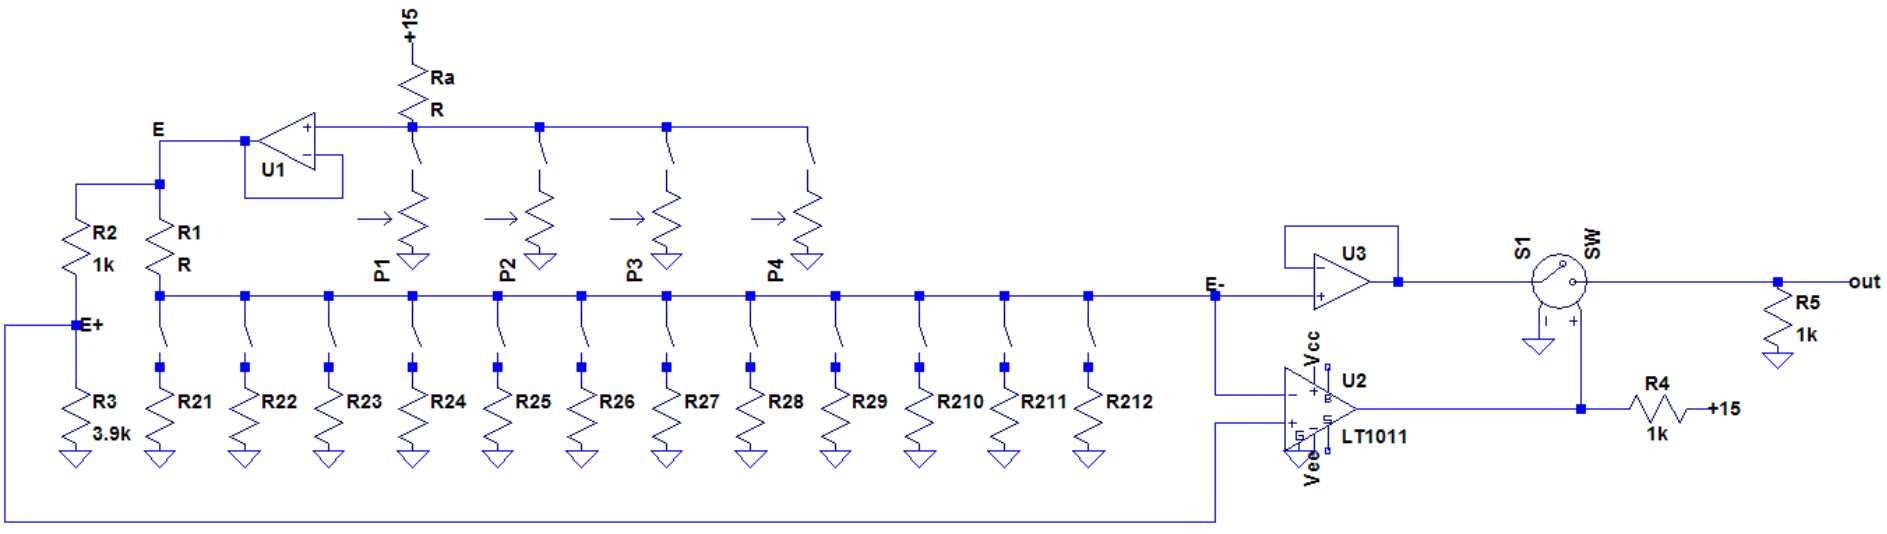
\includegraphics[scale=0.35]{img-keyboard/keyboard-circuit.png}
	\caption{Circuit du clavier. Dans un souci de lisibilité, les valeurs
	des résistances et des potentiomètres n'ont pas été indiquées sur ce
	schémas.}
	\label{fig:keyboard-circuit}
\end{figure}

Le premier réseau de diviseurs résistifs est constitué
de potentiomètres afin de permettre un calibrage des niveaux
de tensions $E$ (et donc de pallier les imprécisions de l'alimentation
\unit{+15}{\volt}). C'est en effet principalement ce paramètre qui
détermine la précision du clavier. Les interrupteurs constituant
ce premier réseau sont des interrupteurs à glissière.
Le tableau \ref{tab:dim-keyboard-first-bloc} résume
le dimensionnement de ce premier bloc.

\begin{table}[ht]
	\centering
	\begin{tabular}{|c|c|}
			\hline
				Résistance & Valeur (en\unit{}{\kilo\ohm}) \\
			\hline
				$R_a$ & 0.47 \\
			\hline
				$P_1$ (octave 8) & maximum 10 \\
			\hline
				$P_2$ (octave 7) & maximum 1 \\
			\hline
				$P_3$ (octave 6) & maximum 0.47 \\
			\hline
				$P_4$ (octave 5) & maximum 0.1 \\
			\hline
		\end{tabular}
	\caption{Résumé du dimensionnement du premier bloc.}
	\label{tab:dim-keyboard-first-bloc}
\end{table}

Le clavier des notes considéré ici comprend 12 touches, 
une pour chaque note et sa dièse correspondante. Les boutons
utilisés sont cette fois des boutons poussoirs.
Pour dimensionner ce bloc, il suffit d'appliquer la
formule suivante 

\[ \text{out} = E\frac{R_{2i}}{R_{2i} + R_1} \text{  avec  } i = 1\dots12. \]

Le dimensionnement complet du clavier se base
sur cette formule. En dimensionnant dans un premier
temps le clavier pour l'octave 8, l'obtention
de l'octave 7 est immédiate en divisant la tension
$E$ par deux, et ainsi de suite pour l'octave 6 et 5.

Le tableau \ref{tab:keyboard-dim} résume les résultats du dimensionnement
du clavier. Seules les valeurs standard de la série de Renard
E12 ont été utilisées. En utilisant une combinaison de 3
résistances en séries ou en parallèles, une erreur inférieure
à 0.01\% est garantie (sans tenir compte des tolérances des
résistances). En utilisant une combinaison plus économique
de seulement 2 résistances, des erreurs bien plus grandes
peuvent survenir (de l'ordre de 0.10\% à 0.30\%). Une telle
erreur est encore raisonnable pour l'oreille humaine qui ne
peut pas différencier deux sons dont la fréquence ne diffère
pas de plus de 0.6\%\cite{frequency-jnd}. Cependant, ces erreurs
risquent encore d'être amplifiées dans les blocs suivant du
synthétiseur, il est donc préférable de les minimiser au maximum
dans ce premier bloc.

\begin{table}[ht]
	\centering
		\begin{tabular}{|c|c|}
			\hline
				Résistance & Valeur (en\unit{}{\kilo\ohm}) \\
			\hline
				$R_1$ & 10 \\
			\hline
				$R_{21}$ (Do) & 2.7 + (1.8 | 12) \\
			\hline
				$R_{22}$ (Do\#) & 0.056 + (4.7 | 180) \\
			\hline
				$R_{23}$ (Ré) & 220 | (0.470 + 4.7) \\
			\hline
				$R_{24}$ (Ré\#) & 4.7 + (0.820 | 270) \\
			\hline
				$R_{25}$ (Mi) & 8.2 | 39 | 56 \\
			\hline
				$R_{26}$ (Fa) & 150 | (0.150 + 6.8)\\
			\hline
				$R_{27}$ (Fa\#) & 100 | 220 | 8.2 \\
			\hline
				$R_{28}$ (Sol) & 15 | 1000 | 18 \\
			\hline
				$R_{29}$ (Sol\#) & 22 | (0.330 + 15) \\
			\hline
				$R_{210}$ (La) & 10 + (0.120 | 2.7)\\
			\hline
				$R_{211}$ (La\#) & 3.3 + (680 | 8.2)\\
			\hline
				$R_{212}$ (Si) & 82 | (15 + 0.390)\\
			\hline
		\end{tabular}
	\caption{Résumé du dimensionnement du clavier.}
	\label{tab:keyboard-dim}
\end{table}

La présence d'un amplificateur suiveur entre le premier
réseau de diviseurs résistifs et le suivant est indispensable
pour les rendre indépendants.

Enfin, le comparateur et le switch présent sur la figure
\ref{fig:keyboard-circuit} fonctionne comme décrit dans la
section précédente.

\section{Confrontations théories et mesures}
Le tableau \ref{tab:keyboard-measure-vs-theory} donne quant
à lui les valeurs mesurées de la tension out. Les imprécisions
s'expliquent par les imprécisions des résistances et/ou du
calibrage.

\begin{table}[ht]
	\centering
		\begin{tabular}{|c|c|c|c|c|}
			\hline
				\specialcell{Octave $\rightarrow$ \\ Note $\downarrow$} & 5 & 6 & 7 & 8 \\
			\hline
				 Do & \unit{510}{\milli\volt} (-2.53\%) & \unit{1040}{\milli\volt} (-0.62\%) & \unit{2100}{\milli\volt} (+0.33\%) & \unit{4160}{\milli\volt} (-0.86\%) \\
			\hline
				 Do\# & \unit{547}{\milli\volt} (-1.26\%) & \unit{1100}{\milli\volt} (-0.78\%) & \unit{2230}{\milli\volt} (-0.58\%) & \unit{4460}{\milli\volt} (-0.565\%) \\
			\hline
				 Ré &  \unit{570}{\milli\volt} (-2.95\%) & \unit{1180}{\milli\volt} (+0.45\%) & \unit{2390}{\milli\volt} (+1.73\%) & \unit{4720}{\milli\volt} (+0.45\%) \\
			\hline
				 Ré\# & \unit{590}{\milli\volt} (-5.18\%) & \unit{1240}{\milli\volt} (-0.36\%) & \unit{2510}{\milli\volt} (+0.84\%) & \unit{4950}{\milli\volt} (-0.56\%) \\
			\hline
				 Mi & \unit{640}{\milli\volt} (-2.92\%) & \unit{1305}{\milli\volt} (-1.02\%) & \unit{2640}{\milli\volt} (+0.11\%) & \unit{5200}{\milli\volt} (-1.40\%) \\
			\hline
				 Fa & \unit{680}{\milli\volt} (-2.64\%) & \unit{1390}{\milli\volt} (-0.49\%) & \unit{2790}{\milli\volt} (-0.14\%) & \unit{5500}{\milli\volt} (-1.56\%) \\
			\hline
				 Fa\# & \unit{720}{\milli\volt} (-2.70\%) & \unit{1470}{\milli\volt} (-0.67\%) & \unit{2950}{\milli\volt} (-0.34\%) & \unit{5840}{\milli\volt} (-1.35\%) \\
			\hline
				 Sol & \unit{770}{\milli\volt} (-1.78\%) & \unit{1560}{\milli\volt} (-0.51\%) & \unit{3140}{\milli\volt} (+0.13\%) & \unit{6180}{\milli\volt} (-1.46\%) \\
			\hline
				 Sol\# & \unit{830}{\milli\volt} (-0.07\%)& \unit{1660}{\milli\volt} (-0.07\%) & \unit{3350}{\milli\volt} (+0.8\%) & \unit{6600}{\milli\volt} (-0.6\%) \\
			\hline
				 La & \unit{860}{\milli\volt} (-2.27\%) & \unit{1750}{\milli\volt} (-0.57\%) & \unit{3510}{\milli\volt} (-0.28\%) & \unit{6940}{\milli\volt} (-1.42\%) \\
			\hline
				 La\# & \unit{915}{\milli\volt} (-1.86\%) & \unit{1850}{\milli\volt} (-0.79\%) & \unit{3730}{\milli\volt} (+0.02\%) & \unit{7380}{\milli\volt} (-1.05\%) \\
			\hline
				 Si & \unit{970}{\milli\volt} (-1.79\%) & \unit{1960}{\milli\volt} (-0.78\%) & \unit{3960}{\milli\volt} (+0.22\%) & \unit{7790}{\milli\volt} (-1.42\%) \\
			\hline
		\end{tabular}
	\caption{Résumé des mesures effectués avec erreur relative calculées par comparaison avec
	le tableau suivant \url{http://fr.wikipedia.org/wiki/Note_de_musique}.}
	\label{tab:keyboard-measure-vs-theory}
\end{table}

Pour améliorer la précision du clavier, plusieurs pistes :
\begin{itemize}
	\item Utiliser des potentiomètres à la place des combinaisons
	de résistances, et calibrer le clavier avant chaque utilisation.
	Cependant cette solution n'est ni économique (un potentiomètre
	coûte beaucoup plus cher qu'une résistance) ni pratique (nécessitera
	un long calibrage) ;
	\item Utiliser des résistances plus précises ($\pm$ 1\% par exemple) ;
	\item Mesurer chaque résistance utilisée et remplacer celles dont la
	valeur est trop imprécise par une autre plus précise.
\end{itemize}
\chapter{L'oscillateur contrôlé en tension (VCO)}
\label{chap:vco}
Le VCO est la partie qui s'occupe de générer un signal périodique à partir d'une tension continue. 
La fréquence du signal généré dépend de manière linéaire à la tension d'entrée avec comme relation
tension-fréquence : \unit{1}{\milli\volt} correspond à \unit{1}{\hertz}. Le comportement
souhaité du VCO est représente sur la figure \ref{fig:in-out-vco}.

\begin{figure}[ht]
	\centering
	\includegraphics[scale=0.3]{img-vco/in-out.png}
	\caption{Relation entrée-sortie souhaitée du VCO.}
	\label{fig:in-out-vco}
\end{figure}

\section{Fonctionnement et théorie}
La figure \ref{fig:schema_bloc_vco} montre le schéma-bloc du VCO.

\begin{figure}[ht]
	\centering
	\includegraphics[scale=0.3]{img-vco/schema_bloc_vco.png}
	\caption{Schéma bloc du VCO.}
	\label{fig:schema_bloc_vco}
\end{figure}

Le VCO est composé des 3 blocs suivants :
\begin{itemize}
	\item le contrôleur de l'intégrateur qui se compose lui-même d'un switch et d'un sommateur.
	\item l'intégrateur.
	\item le trigger de Schmitt (bascule à hystérèse).
\end{itemize}

Le signal d'entrée $in$ est constant et vaut $\alpha$. Soient $V_L$ la
tension de basculement inférieure du trigger, $V_H$ la tension de 
basculement supérieure et $V_{CC}$ la tension d'alimentation du trigger.
Si la sortie du trigger de Schmitt (\textit{contrôle} sur la figure \ref{fig:schema_bloc_vco}) 
vaut $0$, la sortie du switch vaut $0$. Dès lors, la sortie du bloc contrôleur de l'intégrateur vaut $-\alpha$. Après passage dans l'intégrateur, nous avons la 
droite $-K\alpha t$ avec $K$ la constante de temps de l'intégrateur. La sortie du trigger
restera à $0$ tant que la sortie de l'intégrateur est supérieure à $V_L$. Lorsque la sortie
de l'intégrateur atteint $V_L$, le trigger bascule et sa tension de sortie devient $V_{CC}$. 
Le switch change d'état et sa sortie devient $\alpha$. La sortie dû contrôleur de l'intégrateur
devient donc $\alpha$. Après passage dans l'intégrateur, $\alpha$ devient $K\alpha t$. 
La sortie du trigger restera à $V_{CC}$ tant que la sortie de l'intégrateur est inférieure à $V_H$.
Lorsque la sortie de l'intégrateur atteint $V_H$, le trigger bascule et sa tension de sortie devient
$0$. Le switch change à nouveau d'état, sa sortie devient $0$ et le cycle recommence.

La fréquence générée par le VCO pour une tension d'entrée $\alpha$ s'exprime 
en fonction de $K$ et de $\Delta V = \vert V_H - V_L\vert $ par la relation 
\[ f = \frac{K\alpha}{2\Delta V}. \]
L'amplitude du signal généré par le VCO est compris entre $V_H$ et $V_L$.


\section{Dimensionnement et circuit réel}
\paragraph{Circuit réel}
Sur la figure \ref{fig:circuit_vco} se trouve l'implémentation électronique du VCO décrit ci-dessus.

\begin{figure}[ht]
	\centering
	\includegraphics[scale=0.3]{img-vco/vco_circuit}
	\caption{Circuit du VCO}
	\label{fig:circuit_vco}
\end{figure}

\paragraph{Dimensionnement du trigger de Schmitt}
Le choix de placer le seuil supérieur $V_H$ à \unit{0}{\volt} 
et le seuil inférieur $V_L$ à \unit{-1}{\volt} est arbitraire. 
Cependant, la différence entre $V_H$ et $V_L$ doit rester au-dessus
de \unit{500}{\milli\volt} pour éviter une influence des tensions parasites.
% FIX : pas vraiment justifable, 500mV >> quelques mV des tensions parasites.
% On pourrait sans doute encore descendre plus bas.
Dans ce circuit, un trigger asymétrique est utilisé. Dès lors, le rapport
des résistances à utiliser se déduit des formules suivantes : 
\[ V_H = V_{REF}\left(1+\frac{R_2}{R_6}\right) \text{ et } V_L = V_{REF} + \frac{R_2}{R_6}\left(V_{REF}-V_{CC}\right). \]
Dans le montage du trigger asymétrique utilisé, $V_{REF}$, la tension à l'entrée
inverseuse du comparateur vaut \unit{0}{\volt}. Dès lors, $\frac{R_2}{R_6}=\frac{1}{15}$
avec la condition que $R_6 >> R_9$. Les valeurs de résistances choisies sont :

\begin{itemize}
	\item \unit{10}{\kilo\ohm} pour $R_2$ .
	\item \unit{150}{\kilo\ohm} pour $R_6$.
\end{itemize}

\paragraph{Dimensionnement de l'intégrateur}
Calculons maintenant la constante ($K$) du bloc intégrateur. 
Comme le signal de sortie est un signal triangulaire, le temps de montée et de descente est 
identique. Le temps de montée vaut donc $\frac{1}{2\cdot1} = \unit{0.5}{\second}$. 
La pente de montée de la droite est de \unit{1}{\milli\volt}/\unit{}{\second}. 
Le temps pour monter ou descendre de \unit{1}{\volt} est de \unit{1000}{\second}. 
Comme il doit valoir \unit{0.5}{\second}, la constante d'intégration vaut 2000. D'où 
$K=\frac{1}{R_1C_1} = 2000$ avec $C_1= \unit{100}{\nano\farad}$, $R_1 = \unit{5}{\kilo\ohm}$.
\paragraph{Dimensionnement du contrôleur de l'intégrateur}
Le contrôleur de l'intégrateur est constitué d'un amplificateur opérationnel 
en mode différentiel et d'un switch. L'équation constitutive de ce bloc est : 
$V_{IC}=2*V_+ - V_-$ avec $V_+$ la tension à l'entrée non-inverseuse et $V_-$
la tension à l'entrée inverseuse. La formule suivante permettant de déterminer
une relation entre les résistances est obtenue en appliquant KCL : 
\[ V_{IC}=V_+ \left(\frac{R_4 + R_5}{R_5}\right)-V_-\left(\frac{R_4}{R_5}\right). \] 
Cela donne donc $R_5 = R_4$. En prenant $R_5 =$ \unit{1}{\kilo\ohm}, $R_4$ vaut \unit{1}{\kilo\ohm}
et $R_3$ vaut \unit{10}{\kilo\ohm}.

\section{Confrontation  des mesures et de la théorie}
La figure \ref{fig:theory_vs_mesure} montre que la réalité est la théorie sont très proche.
Les différences observées sont dues à des imprécisions des valeurs des résistances et des 
capacités. Cela provient aussi du switch qui contrairement au modèle utilisé dans les 
simulations et les calculs possède une légère courbe d'hystérèse.
\begin{figure}
	\centering
	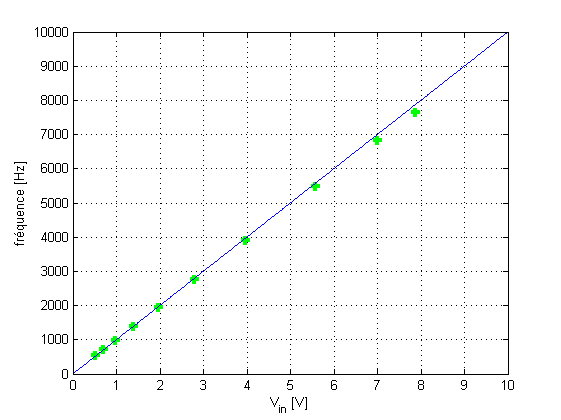
\includegraphics[scale=0.45]{img-vco/vco_vs_reality.png}
	\caption{Confrontations des théories et des mesures.}
	\label{fig:theory_vs_mesure}
\end{figure}
\chapter{Filtre}
\label{sec:filtre}
Le MLI a besoin d'un signal sinusoïdal pour fonctionner, cependant, le VCO fournit un
signal triangulaire. Il est donc nécessaire d'avoir un filtre intermédiaire permettant
de transformer le signal de sortie du VCO en signal sinusoïdal ou tout du moins pseudo-sinusoïdal.
L'objectif de ce filtre est donc d'obtenir un graphe d'entrée-sortie similaire à
celui présenté sur la figure \ref{fig:filter-in-out}.

% TODO : refaire ce graphe avec les bon titres
\begin{figure}[ht]
	\centering
	\includegraphics[scale=0.4]{img-filter/in-out.png}
	\caption{Entrée et sortie du filtre : objectif.}
	\label{fig:filter-in-out}
\end{figure}

\section{Fonctionnement}

\begin{figure}[ht]
	\centering
	\includegraphics[scale=0.4]{img-filter/circuit-colored.png}
	\caption{Circuit du filtre.}
	\label{fig:circuit-filtre}
\end{figure}

Le filtre utilise des diodes pour faire varier le circuit en fonction de la tension d'entrée. 
Le circuit possède ainsi 4 états différents selon sa tension d'entrée :
\begin{enumerate}
	\item Elle est trop basse pour traverser la moindre diode :\\
				Dans ce cas-ci, seule la partie bleue du circuit est active, 
				il n'y a pas de courant, la tension d'entrée est don égale à
				la tension de sortie ;
	\item Elle est suffisante pour traverse une diode :\\
				Ici, la partie rouge du circuit (voir figure \ref{fig:circuit-filtre} est active. 
				On se retrouve donc avec un diviseur de tension qui diminuera la tension de sortie par rapport à la valeur d'entrée ;
	\item Elle est suffisante pour traverser deux diodes :\\
				La partie orange s'active en plus, ce qui mettra en parallèle les resistances $R_1$ et $R_2$ et
				réduira donc encore d'avantage la tension de sortie ;
	\item Elle est suffisante pour être écrêter par trois diodes :\\
				À partir d'ici, la résistance interne des 3 diodes jaunes va se mettre en parallèle avec $R_1$ et $R_2$
				\footnote{Si les diodes étaient idéales,
				le circuit fonctionnerait moins bien : au lieu d'obtenir un sommet de courbe de tension 
				arrondi dû à la résistance dynamique des diodes, on aurait un sommet de courbe
				horizontal à cause du lien direct à la masse. On pourrait cependant rajouter une résistance
				$R_3$ très faible derière les diodes pour redresser légèrement le sommet de la courbe.}. Étant donné que la 
				resistance interne des diodes est très faible comparée à $R_0$, il n'y a que peu de tension
				qui s'ajoutera encore à la tension de sortie.
\end{enumerate}

\section{Détails du circuit}
\begin{enumerate}
	\item Signal d'entrée :\\
				Le signal d'entrée doit être suffisament grand pour commencer à être
				écrêter par trois diodes en série, le signal de sortie culminera donc
				aux alentours de \unit{1.9}{\volt}. Le signal d'entrée est donc le signal
				triangulaire circonscrit au signal sinusoïdal d'amplitude \unit{1.9}{\volt},
				soit un signal triangulaire d'amplitude \unit{3}{\volt}\footnote{Comme expliqué
				dans le chapitre \ref{chap:vco}, la sortie du VCO est un triangle compris entre
				\unit{-1}{\volt} et \unit{0}{\volt}. Un bloc supplémentaire comprenant un filtre
				passe haut (afin de supprimer la composante continue) et un amplificateur opérationnel
				(pour amplifier le signal) a donc été ajouté après le VCO.} ;
	\item Valeur des résistances : \\
		\begin{enumerate}
			\item Première approximation : $R_0$ a été définie à \unit{1}{\kilo\ohm}. $R_1$ quant à lui
						a été défini à \unit{7.9}{\kilo\ohm} afin que la pente de la tension avec 
						le diviseur $R_0$/$R_1$ soit égale à la pente moyenne de $y = 1.9\sin{Cx}$ entre $y=0.6$
						et $y = 1.2$ (soit $0.87C$). $R_2$ vaut \unit{2.2}{\kilo\ohm} afin que la pente de la 
						tension avec le diviseur $R_0$/($R_1$//$R_2$) soit égale à la pente moyenne de $y = 1.9\sin{Cx}$
						entre $y = 1.2$ et $y = 1.8$ (soit $0.58C$)

						Avec cette première approximation, le taux de distortion harmonique total est compris entre 0.51\% 
						(\unit{500}{\hertz}) et 0.5\%(\unit{10}{\kilo\hertz}).
			\item Seconde approximation : pour améliorer ensuite le pseudo-sinus, des tests empiriques ont amené
						à une valeur de \unit{12.1}{\kilo\ohm} pour $R_1$ et de \unit{2.1}{\kilo\ohm} pour $R_2$.\\
						Avec ces nouvelles valeurs, le taux de distortion harmonique total est compris entre 0.3\% 
						(\unit{500}{\hertz}) et 0.23\% (\unit{10}{\kilo\hertz}). Les FFT
						théoriques (réalisées avec LTSpice) du signal d'entrée, du signal de sortie et d'un sinusoïdale
						pure sont présentées sur la figure \ref{fig:fft-filtre}.
		\end{enumerate}
\end{enumerate}

\begin{figure}[ht]
	\centering
	\includegraphics[scale=0.4]{img-filter/FFT.png}
	\caption{FFT avec les résistances de la seconde estimation.}
	\label{fig:fft-filtre}
\end{figure}

\section{Confontation théorie et mesures}

\begin{figure}[ht]
	\centering
	\includegraphics[scale=0.6]{img-filter/THD.png}
	\caption{Confrontation THD réel et théorique}
	\label{fig:thd-filtre}
\end{figure}

Dans la pratique, le TDH\footnote{Pour taux de distortion harmonique.} 
est non seulement beaucoup plus important que dans la réalité, mais aussi beaucoup plus 
variable (voir figure \ref{fig:thd-filtre}). Cela est principalement dû au manque de précision des composants dans le filtre
et en amont\footnote{En effet, cela cause une imprécision dans le signal d'entrée du filtre
qui n'est pas exactement un signal triangulaire \unit{+3}{\volt}/\unit{-3}{\volt}}. Mais c'est
aussi dû aux glitchs provoqués par le MLI qui perturbent le pseudo-sinus.

\section{Améliorations possibles}

\begin{enumerate}
	\item Coder un programme capable de calculer avec précision $R_0$, $R_1$, $R_2$ et la tension 
				d'entrée afin de réduire au maximum le taux de distortion harmonique ;
	\item S'arranger pour que les données pratiques soient plus proches des données théoriques afin 
				de minimiser l'erreur dûe à la tolérance des composants.
\end{enumerate}
\chapter{Modulateur sigma-delta}
\label{sec:sigma-delta}
Le modulateur sigma-delta se trouve à la suite du filtre et avant l'amplificateur de classe D. 
Ce bloc a pour but de moduler le signal d'entrée (un pseudo sinus) par largeur d'impulsion,
c'est-à-dire en signal carré de valeurs seuils constantes mais de fréquence variable dont la
valeur moyenne est égale à la valeur absolue du signal initial. L'obtention d'un signal composé
de deux états est nécessaire pour une utilisation optimale en terme de puissance de l'amplificateur de classe D.

\begin{figure}[ht]
	\centering
	\includegraphics[scale=0.7]{img-sigma-delta/in-out.png}
	\caption{Entré et sortie du sigma-delta}
	\label{fig:entrée-sortie-sigma-delta}
\end{figure}

\section{Fonctionnement du système}
La fréquence de commutation du sigma-delta est supposée très élevée par rapport
au signal d'entrée. Ceci permet de considérer le signal d'entrée constant localement.

Voici ci-dessous le schéma bloc du sigma-delta.

\begin{figure}[ht]
	\centering
	\includegraphics[scale=0.7]{img-sigma-delta/schema-blocs.png}
	\caption{Schéma bloc du modulateur sigma-delta (source : Bruno Dehez).}
	\label{fig:sigma-delta-schema-blocs}
\end{figure}

Ce bloc est constitué de deux parties distinctes : un intégrateur et une bascule asymétrique.
L'intégrateur est caractérisé par un coefficient d'intégration K. La bascule est elle caractérisée
par deux tensions de basculement : $V_H$, la tension de basculement haute fixée arbitrairement à 0 
et $V_L$, la tension de basculement basse avec $\Delta V = V_H - V_L$, ainsi que des valeurs seuils
de sortie : $V_{\text{outH}} = E$, la tension de sortie haute, et la tension $V_{\text{outL}} = 0$. 
$V_{\text{outL}}$ est fixée à 0 car l'amplificateur de classe D nécessite en entré une tension positive ($E$), ou 0.

La période d'oscillation du signal de sortie (qui est 
identique à la période d'oscillation du signal intermédiaire
$V_I$ sur la figure \ref{fig:sigma-delta-schema-blocs})
se calcule en effectuant le raisonnement suivant.
Initialement, soit $V_{\text{ref}}$ positif et
$V_{\text{out}} = 0$. $V_I$ est alors immédiatement positif
et $V_{\text{out}}$ sature directement à $E$. Comme $V_{\text{ref}}$
est $\leq E$, $V_I$ va maintenant décroître jusqu'à atteindre
$\Delta V$. A ce moment précis, $V_{\text{out}} = 0$
et donc $V_I$ va croître jusqu'à atteindre 0, et ainsi de suite.

De là s'obtiennent le temps de descente $t_f$ et le temps de montée $t_r$
du signal $V_I$\footnote{Ce signal sera soit un signal triangulaire,
soit un signal en dents de scie, selon la valeur de $V_{\text{ref}}$.}
\[ t_f = -\frac{\Delta V}{(V_{\text{ref}} - E)K},\]
\[ t_r = \frac{\Delta V}{KV_{\text{ref}}}.\]
La période $T$ étant la somme du temps de descente et du temps
de montée, elle est donnée par
\[ T = \frac{\Delta V}{K}\left(\frac{1}{V_{\text{ref}}} - \frac{1}{V_{\text{ref}} - E}\right) \]
et donc finalement
\begin{equation} 
	f = -\frac{K}{\Delta V} \frac{V_{\text{ref}}(V_{\text{ref}}-E)}{E}.
	\label{eq:sigma-delta-frequency}
\end{equation}

\paragraph{Remarque}
A partir du temps de descente et du temps de montée, nous
pouvons prouver que la moyenne du signal carré $V_{\text{out}}$
vaut bien $V_{\text{ref}}$. Il suffit de démontrer l'égalité
suivante
\[ \frac{E \cdot t_f + 0 \cdot t_r}{T} = V_{\text{ref}}.\]

La fréquence en fonction de $V_{\text{ref}}$ est donc
une parabole avec une racine en \unit{0}{\volt} et une
racine en \unit{E}{\volt}.

La fréquence de sortie maximale est atteinte pour 
$V_{\text{ref}} = \frac{E}{2}$ et vaut
\[ f_{\text{max}} = \frac{K}{\Delta V}\frac{E}{4}. \]
Le sigma-delta doit remplir certaines spécifications afin de remplir son rôle au sein du système global : 
\begin{enumerate}
	\item Le signal de sortie ne peut pas atteindre de fréquence nulle pour la gamme d'amplitude du signal
	d'entrée car la valeur moyenne du signal de sortie ne correspondrait pas au signal d'entrée pour ces deux racines ;
	\item La fréquence de sortie du sigma-delta doit respecter le théorème d’échantillonnage de Shannon, c'est-à-dire
	que la fréquence de sortie doit être au minimum deux fois supérieure à la fréquence maximale du signal d'entrée
	afin de permettre la reconstitution du signal d'entrée ;
	\item La fréquence maximale d'entrée de l'amplificateur de classe D est de \unit{100}{\kilo\hertz} ;
	\item La bascule ne doit pas être sensible au bruit, $\Delta V$ ne doit donc pas être trop faible.
\end{enumerate}

Afin de répondre à ces conditions, la fréquence maximale de sortie est fixée à \unit{80}{\kilo\hertz},
de telle sorte que :
\[ \frac{K}{\Delta V}\frac{E}{4} = 80000. \]

La parabole de l'équation \ref{eq:sigma-delta-frequency} est centrée autour de l'origine car le signal
d'entrée est centrée en 0 et les racines de celles-ci se situent en \unit{+15}{\volt} et \unit{-15}{\volt}. 
Ainsi, la gamme d'amplitude de tension d'entrée étant de \unit{-3}{\volt} à \unit{3}{\volt} 
la fréquence de sortie n'est jamais nulle. De plus, la fréquence maximale du signal d'entrée étant de \unit{8}{\kilo\hertz}, 
la fréquence du signal de sortie est bien supérieure au double de cette fréquence pour l'ensemble de la gamme d'amplitude. 
$V_{\text{ref}}$ est fixé arbitrairement à $1V$.

La figure ci-dessous illustre la réponse en fréquence établie et met en évidence la limite induite par le 
théorème de Shannon ainsi que la gamme utilisée par notre système.

\begin{figure}[ht]
	\centering
	\includegraphics[scale=0.5]{img-sigma-delta/sigma-delta-lim.png}
	\caption{Fréquence de sortie en fonction de la tension d'entrée et contraintes}
	\label{fig:sigma-delta-lim}
\end{figure}

Il est possible de constater que la zone utilisée est nettement inférieure à la zone exploitable. 
Cela sera mis plus en avant dans la section \ref{sec:pistes-amelioration}.

\section{Dimensionnement et circuit réel}
Le circuit du modulateur sigma-delta est représenté
à la figure \ref{fig:sigma-delta-circuit}.

\begin{figure}[ht]
	\centering
	\includegraphics[scale=0.65]{img-sigma-delta/sigma-delta-circuit.png}
	\caption{Circuit du modulateur.}
	\label{fig:sigma-delta-circuit}
\end{figure}

La résolution de ce circuit permet d'obtenir des équations
de la même forme que celles de la figure
\ref{fig:sigma-delta-schema-blocs}.
L'amplificateur opérationnel étant connecté en contre-réaction,
sa bornée d'entrée est virtuellement à la masse : $v_- = v_+ = 0$.
Les différents courants dans le circuit sont alors donnés par
\[ i_{R_4} = \frac{V_{\text{ref}}}{R_4},\]
\[ i_{R_6} = \frac{V_{\text{ee}}}{R_6},\]
\[ i_{R_3} = \frac{V_{\text{out}}}{R_3},\]
\[ i_{C_1} = -C_1\fdif{v_{\text{in}}}{t}.\]
KCL permet ensuite d'écrire l'équation suivante
\[ i_{C_1} = i_{R_4} + i_{R_6} + i_{R_3}\]
et donc d'obtenir
\[ v_{\text{in}} = -\frac{1}{C_1}\int \frac{V_{\text{ref}}}{R_4}
+ \frac{V_{\text{ee}}}{R_6} + \frac{V_{\text{out}}}{R_3}.\]
Pour se ramener à l'équation de la figure
\ref{fig:sigma-delta-schema-blocs}, on
$V'_{\text{ref}} = -R_3(\frac{V_{\text{ref}}}{R_4}+\frac{V_{\text{ee}}}{R_6})$
pour enfin obtenir
\[ v_{\text{in}} = \frac{1}{C_1R_3} \int V'_{\text{ref}} - V_{\text{out}}\]
où $V'_{\text{ref}}$ correspond au $V_{\text{ref}}$
de la figure \ref{fig:sigma-delta-schema-blocs}.

Pour centrer la parabole, il faut que $\frac{R_3}{R_6}V_{\text{ee}}$
soit égale à \unit{6.75}{\volt}. Il faut ensuite étirer la
parabole de manière à ce que ses racines soient $\pm$\unit{15}{\volt}.
Il faut donc $\frac{R_3}{R_4} = 0.45$. 

En utilisant des valeurs de composants standards (série de Renard E12), 
nous pouvons choisir, $R_3 =$ \unit{22}{\kilo\ohm} et $R_4 = R_6 =
$ \unit{48.5}{\kilo\ohm}.

Passons ensuite à la contrainte sur la fréquence. Nous avons la 
relation suivante:
\[ \frac{K}{\Delta V}\frac{E}{4} = 80000.\]
Nous pouvons fixer arbitrairemet $\Delta V$ à \unit{1}{\volt}. Nous avons alors
$K = \frac{1}{C_1R_3} = 23703.7037$ et donc $C1 =$ \unit{1.9}{\nano\farad}.
Enfin, comme $\Delta V = \frac{R_1}{R_2}E$, nous pouvons par exemple
choisir $R_1 =$ \unit{10}{\kilo\ohm} et $R_2 =$ \unit{134.6}{\kilo\ohm}.

Pour appliquer la signal de sortie du modulateur
à l'étage suivant du circuit, il faudra utiliser un diviseur
résistif car l'étage suivant ne supporte pas des entrées supérieures
à \unit{5}{\volt}.

\section{Confrontation des mesures et de la théorie}
En superposant le graphe théorique que nous pouvons obtenir avec les valeurs
obtenues dans la section précédente
et des mesures effectuées sur une implémentation en circuit
du modulateur, nous obtenons la figure \ref{fig:sigma-delta-f-vs-vref-dim-vs-real}.

\begin{figure}[ht]
	\centering
	\includegraphics[scale=0.70]{img-sigma-delta/sigma-delta-f-vs-vref-dim-vs-real.png}
	\caption{En bleu, les prévisions théoriques et en vert les mesures.}
	\label{fig:sigma-delta-f-vs-vref-dim-vs-real}
\end{figure}

Cette figure révèle que la théorie colle assez bien à la réalité. Le
faible décalage dépend sans doute des tolérances des résistances,
des variations dans les alimentations ou encore de la précision des
circuits intégrés.
\chapter{Système global}
Après avoir décrit chaque bloc de façon individuelle, il est nécessaire d'observer le système dans son ensemble afin de pouvoir valider, ou non, son bon fonctionnement. 

\section{Assemblage}
Il est important que chacun des blocs se comportent au sein
du système global comme défini dans les sections précédentes, 
autrement dit : que les blocs n'interfèrent pas entre eux.
Pour cela, il est possible d'ajouter des amplificateurs 
opérationnels en suiveur\footnote{Idéalement, les amplificateurs opérationnels
ont une impédance d'entrée infinie et une impédance de sortie nulle.} 
entre les blocs afin d'assurer une liaison imperméable. 
%Le premier se trouve entre le filtre sinusoïdale
%et le sigma-delta. En effet, la résistance équivalente du
%sigma-delta n'est pas infini et interfère donc avec le filtre
%si il ne sont pas isolés à l'aide d'un suiveur.
%Les autres blocs ne nécessitent pas d'étage tampon en vue
%de leurs agencements individuels

\section{Validation}
Afin de valider le circuit de façon globale le tableau ci
dessous met en évidence l'erreur en fréquence et le taux de
distortion harmonique observés à la sortie du filtre pour
diverses notes jouées.La validation du sigma-delta est
effectuée grâce à une application \textsc{Android} permettant de
mesurer la fréquence d'un signal audio. Ceci a été effectué
pour l'ensemble des notes, mais le tableaux ne reprend que
quelques valeurs significatives et les maximas. Le clavier a
été calibré avant la prise de mesure.

\begin{table}
	\centering
	\begin{tabular}{|c|c|c|c|}
		\hline
		Clavier &  \multicolumn{2}{c|}{Filtre} &  Sortie audio \\
		 \hline
		Note &  Erreur fréquence (\%) & TDH (\%) &  Erreur fréquence (\%) \\
		\hline
		D5 &  -4.1 & 1.55 & -3.8\\
		B5 &  2.9 & 2.26 & 3.2\\
		F6 &  1.6 & 1.92 & 1.3\\
		F7 &  0.9 & 2.02 & 1.5\\
		C8 &  0.3 & 2.08 & 0.2\\
		F8 &  2.3 & 1.29 & 2.1\\
		\hline
	\end{tabular}
	\caption{Tableau de validation du système global.}
	\label{tab:tab-global}
\end{table}

Cette partie du système remplit bien son rôle. L'erreur en 
fréquence se trouve dans une gamme raisonnable (de -3.8\% à 3.2\%)
sur l'ensemble de la gamme fréquentielle couverte. Les notes 
correspondent donc chaque fois à la note souhaitée, et non à celle
supérieure ou inférieure.
Quant au taux de distortion harmonique, il ne dépasse pas 2.8\%.

Des 'glitchs' apparaissent sur l'ensemble du circuit et ce à 
même fréquence que la fréquence de sortie du sigma-delta. Ceci est dû au fait que
le sigma delta pompe du courant à la source par à coup. Cela ne modifie
que légèrement la qualité du système.

\section{Pistes d'amélioration}
\label{sec:pistes-amelioration}
La conception et la mise en oeuvre de chaque bloc ont été effectué
de manière locale et non globale, des blocs
intermédiaires (adaptateurs) ont dû être ajouté en conséquence. Une vision plus
globale dès le début du projet aurait permis une simplifaction du
système final ainsi qu'une diminution du nombre de composants et
donc de puissance utilisée et d'erreurs possibles.

En pratique, il aurait été possible de modifier la gamme de sortie
du VCO afin que celle-ci corresponde à l'entrée du filtre (
triangle entre \unit{-3}{\volt} et \unit{+3}{\volt}), et donc 
supprimer l'adaptateur. Il faut pour cela modifier les seuils
de basculements de la bascule à hystérèse afin qu'ils soient de
\unit{-3}{\volt} et \unit{+3}{\volt}, et ensuite adapter la
constante d'intégration pour que le lien amplitude d'entrée/fréquence
de sortie soit toujours respecté. D'un point de vue circuit, il s'agit
donc de changer les résistances caractéristiques de la basucle, et le
condensateur nécessaire à l'intégration. Réaliser l'opération inverse,
c'est-à-dire modifier les caractéristiques du filtre afin qu'il accepte
en entrée un signal correspondant à la sortie actuelle du VCO 
(triangle entre \unit{-1}{\volt} et \unit{0}{\volt}) n'aurait pas été 
possible étant donné la conception de celui-ci (voir section \ref{sec:filtre}). 
Pour cela, il est nécessaire de concevoir un nouveau filtre.

Il est également possible de réaliser un clavier dont la sortie serait directement
liée à la masse lorsqu'aucune touche n'est enfoncée, sans nécéssiter un comparateur
et un switch. Cependant cette solution nous échappe encore.ytred

Comme mis en avant dans la section \ref{sec:sigma-delta} concernant le
sigma-delta, le bloc 'sigma-delta' actuel n'utilise qu'une mince zone
de fréquence de commutation. En effet, il serait possible de diminuer
les racines de la parabole de la figure \ref{fig:sigma-delta-lim}, 
afin que la zone de fréquence atteignable pour le signal d'entrée 
(compris entre \unit{-3}{\volt} et \unit{3}{\volt})
soit plus importante toute en s'assurant que la fréquence minimale
atteinte soit au-delà de la fréquence de Shannon (\unit{16}{\kilo\hertz} dans
notre cas). Il suffit de fixer judicieusement les deux tensions d'entrée qui produisent
en sortie un signal dont la fréquence correspond à la fréquence de Shannon. 
Ces points pourraient être fixés à \unit{-4}{\volt} et \unit{4}{\volt}
afin de garder une marge d'erreur. La contrainte sur la fréquence
de sortie maximale reste identique.
Ces trois points donne l'équation de la nouvelle parabole. Une plus 
grande zone de fréquence de commutation permet une meilleure reconstitution
du signal d'entrée.

Concernant les 'glitchs' observés, l'unique solution est d'utiliser deux 
sources d'alimentation distinctes : une pour le sigma-delta, et une pour le reste du circuit.
\chapter{Conclusion}
Au terme de ce quatrième quadrimestre, c'est avec un sentiment de satisfaction
que nous clôturons notre projet. En fabriquant un synthétiseur analogique,
nous avons appris plein de choses et développé de nouvelles compétences.
Tout d'abord, partant de la décomposition du circuit en blocs fonctionnels,
nous avons traduit ces blocs en circuits électriques que nous avons simulé.
Par la suite, nous les avons montés et testés. Et pour finir, nous avons confronté
la théorie, les simulations et la réalité. Nous avons donc acquis la démarche de
conception de circuits électriques.

Le son produit par notre synthétiseur est très proche d'une sinusoïde. Le taux de
distorsion harmonique est au maximum de 3\%. L'erreur maximale sur la fréquence
d'une note est de l'ordre de 3\%. Cette erreur est due aux incertitudes sur les
valeurs des composants utilisés dans le circuit.
L'amplitude du signal de sortie varie très peu sur l'ensemble de la gamme de sortie.
Notre synthétiseur permet de jouer des notes de l'octave 5 à l'octave 8. 
Nous couvrons donc 4 octaves.

La vision par blocs du synthétiseur n'est pas assez globale. Cela nous posa
quelques petits problèmes lors de l'assemblage. Pour résoudre ces problèmes, 
nous avons dû ajouter des adaptateurs entre chaque bloc fonctionnel. Une piste
d'amélioration est donc d'envisager la conception de façon plus globale afin
de ne plus avoir besoin ces adaptateurs. Une autre piste d'amélioration intéressante
est de réduire les perturbations introduite par le MLI sur l'ensemble du signal en 
l'alimentant avec une autre source que le reste du système.

\biblioreport{biblio}

\end{document}